\section{Experiments}
\label{sec:experiments}

We adapt DeepPQR's synthetic study to isolate the effect of identification. DeepPQR already showed that PQR-style recovery can outperform linear DDC baselines, MaxEnt IRL, and AIRL when the target is normalized reward recovery rather than imitation. Our focus is narrower: we compare DeepPQR and GenPQR under matched policy estimation, and study how policy and \(Q\)-estimation choices affect modular reward recovery. We use the infinite-horizon DeepPQR environment with continuous states, five actions, deterministic transitions, and anchor-action normalization with \(g(s)=0\). We report reward mean squared error, reward correlation with the true normalized reward, held-out policy negative log-likelihood, and runtime, averaged over \(100\) seeds with \(95\%\) confidence intervals. Simulator and optimization details are deferred to Appendix~\ref{app:simulation-details}.

\subsection{Matched Comparison to DeepPQR}
\label{sec:experiments:matched}

Our first experiment is a matched comparison in the anchor-action setting. Both methods use the same AIRL policy estimate and neural downstream approximation, so the remaining difference is the identification step. We vary sample size and anchor frequency, which together determine DeepPQR's effective anchor sample size. Table~\ref{tab:exp1_matched} reports three representative regimes, and Figure~\ref{fig:exp1_matched} summarizes the same comparison graphically.

\begin{table}[htb]
\centering
\caption{Matched DeepPQR vs.\ GenPQR comparison. Both methods use the same AIRL policy estimate; GenPQR uses neural FQE. Entries are mean $\pm$ 95\% CI over 100 seeds. Anchor count is the effective sample size for DeepPQR's anchor-$Q$ step.}
\label{tab:exp1_matched}
\scriptsize
\setlength{\tabcolsep}{4pt}
\begin{tabular}{llccccc}
\toprule
Setting & Method & Anchor count & Anchor frac. & Reward MSE $\downarrow$ & Reward corr. $\uparrow$ & Time (s) $\downarrow$ \\
\midrule
Low / rare & DeepPQR & 311 & 0.156 & 2.599 $\pm$ 0.149 & 0.464 $\pm$ 0.029 & 7.33 $\pm$ 0.10 \\
Low / rare & GenPQR (AIRL, neural FQE) & 311 & 0.156 & \textbf{0.912 $\pm$ 0.111} & \textbf{0.659 $\pm$ 0.029} & \textbf{5.22 $\pm$ 0.08} \\
\midrule
Mid / rare & DeepPQR & 1559 & 0.156 & 1.480 $\pm$ 0.095 & 0.611 $\pm$ 0.029 & 38.84 $\pm$ 0.60 \\
Mid / rare & GenPQR (AIRL, neural FQE) & 1559 & 0.156 & \textbf{0.758 $\pm$ 0.077} & \textbf{0.731 $\pm$ 0.024} & \textbf{27.76 $\pm$ 0.42} \\
\midrule
High / common & DeepPQR & 6280 & 0.251 & 0.703 $\pm$ 0.070 & 0.731 $\pm$ 0.023 & 92.82 $\pm$ 1.28 \\
High / common & GenPQR (AIRL, neural FQE) & 6280 & 0.251 & \textbf{0.598 $\pm$ 0.061} & \textbf{0.735 $\pm$ 0.023} & \textbf{64.09 $\pm$ 0.90} \\
\bottomrule
\end{tabular}
\end{table}

\begin{figure}[htb]
\centering
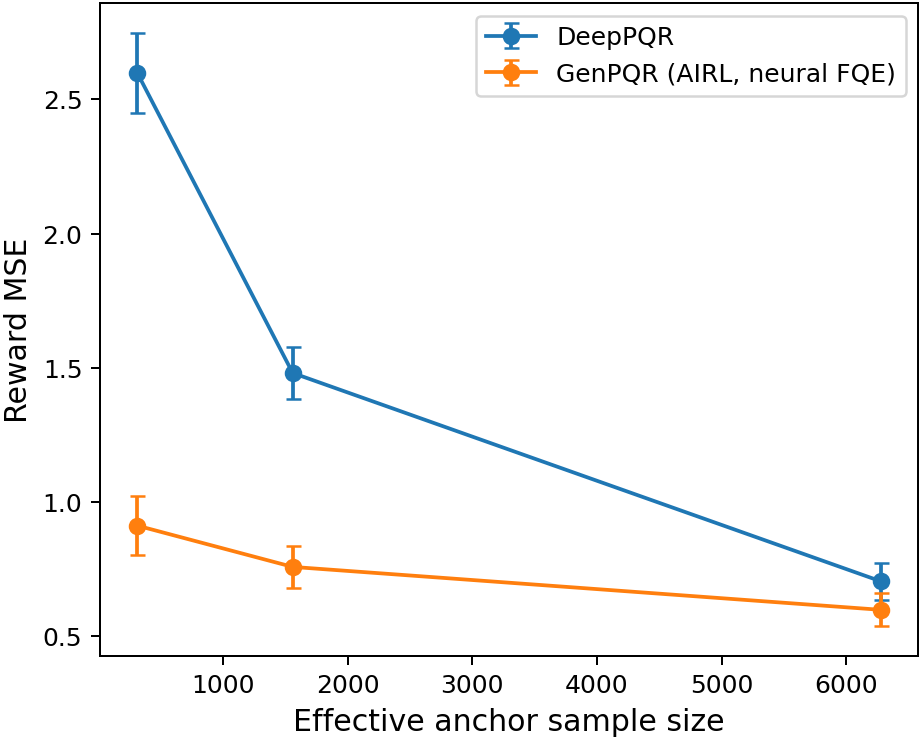
\includegraphics[width=0.95\linewidth]{exp1_matched_curve.png}
\caption{Matched DeepPQR vs.\ GenPQR comparison across anchor-support settings. Points show means and error bars show 95\% confidence intervals over 100 seeds.}
\label{fig:exp1_matched}
\end{figure}

\subsection{Higher-Sample Method Comparison}
\label{sec:experiments:methods}

Our second experiment studies estimator choice in a higher-sample regime with a non-rare anchor action. We compare AIRL versus behavior cloning for policy estimation, neural versus boosted fitted-\(Q\) evaluation, and include DeepPQR and standard reward-recovery baselines. Table~\ref{tab:exp2_methods} shows that the modular GenPQR formulation remains effective across estimator choices, while runtime varies substantially across implementations.

\begin{table}[htb]
\centering
\caption{Higher-sample method comparison. Entries are mean $\pm$ 95\% confidence interval over 100 seeds.}
\label{tab:exp2_methods}
\scriptsize
\setlength{\tabcolsep}{4pt}
\begin{tabular}{lcccc}
\toprule
Method & Reward MSE $\downarrow$ & Reward corr. $\uparrow$ & Policy NLL $\downarrow$ & Time (s) $\downarrow$ \\
\midrule
GenPQR (BC, neural FQE) & \textbf{0.370 $\pm$ 0.059} & \textbf{0.814 $\pm$ 0.011} & \textbf{1.546 $\pm$ 0.004} & 4.74 $\pm$ 0.06 \\
GenPQR (AIRL, neural FQE) & 0.632 $\pm$ 0.064 & 0.717 $\pm$ 0.025 & 1.608 $\pm$ 0.006 & 26.43 $\pm$ 0.34 \\
GenPQR (BC, boosted FQE) & 1.067 $\pm$ 0.189 & 0.493 $\pm$ 0.030 & \textbf{1.546 $\pm$ 0.004} & \textbf{2.25 $\pm$ 0.03} \\
GenPQR (AIRL, boosted FQE) & 1.066 $\pm$ 0.188 & 0.410 $\pm$ 0.049 & 1.608 $\pm$ 0.006 & 23.97 $\pm$ 0.32 \\
\midrule
DeepPQR & 0.794 $\pm$ 0.065 & 0.692 $\pm$ 0.023 & 1.608 $\pm$ 0.006 & 38.24 $\pm$ 0.42 \\
MaxEnt-IRL (Q as reward) & 1.167 $\pm$ 0.177 & 0.351 $\pm$ 0.027 & 1.624 $\pm$ 0.005 & 8.57 $\pm$ 0.11 \\
AIRL state reward & 2.175 $\pm$ 0.215 & -0.006 $\pm$ 0.030 & 1.608 $\pm$ 0.006 & 23.83 $\pm$ 0.32 \\
Log-policy pseudo reward & 3.401 $\pm$ 0.185 & 0.374 $\pm$ 0.047 & 1.608 $\pm$ 0.006 & 23.83 $\pm$ 0.32 \\
\bottomrule
\end{tabular}
\end{table}

Across the two studies, the matched comparison isolates the statistical cost of anchor-subset identification, while the higher-sample comparison shows that GenPQR remains effective across practical estimator choices. Additional details are deferred to Appendix~\ref{app:simulation-details}.
